\documentclass{article}
\usepackage{graphicx}
\usepackage[designiv]{web}
\usepackage{eforms}

\parskip6pt
\parindent0pt

\begin{insDLJS}[_robot]{robot}{AcroRobot JS}
var _robot=true;
/*
    The entries of this array are of two types:
        (1) a string that AcroRobot will speak to the listener;
        (2) a number, which is the number of milliseconds AcroRobot will be silent.
    Sometimes, you have to type a word different so AcroRobot will pronounce it
    close to correct. For example, I used Tech rather than TeX below.
*/
var robotSpeak = new Array(
    "I am your friendly robot man.",500,
    "I can do whatever superman can!",500,
    "Created with the neat tools of AcroTech dot Net.",500,
    "I'll be the best friend you have ever met!",1000,
    "Now, I must get back to my retirement! Enjoy!",1500,
    "dps.",500,
    "I am robot man.",500,
    "beep, beep."
);
function robotTalks()
{
    if ( tts.available ) {
        tts.speaker = tts.getNthSpeakerName(0);
        for ( var i=0; i < robotSpeak.length; i++)
           ( typeof robotSpeak[i] == "string" ) ? tts.qText(robotSpeak[i]) : tts.qSilence(robotSpeak[i]);
        tts.talk();
    }
}
\end{insDLJS}

\pagestyle{empty}

\begin{document}

%\previewtrue

\begin{center}
  \sffamily\bfseries\Large\color{blue}AcroRobot Speaks!
\end{center}
\begin{center}
{\setbox0=\hbox{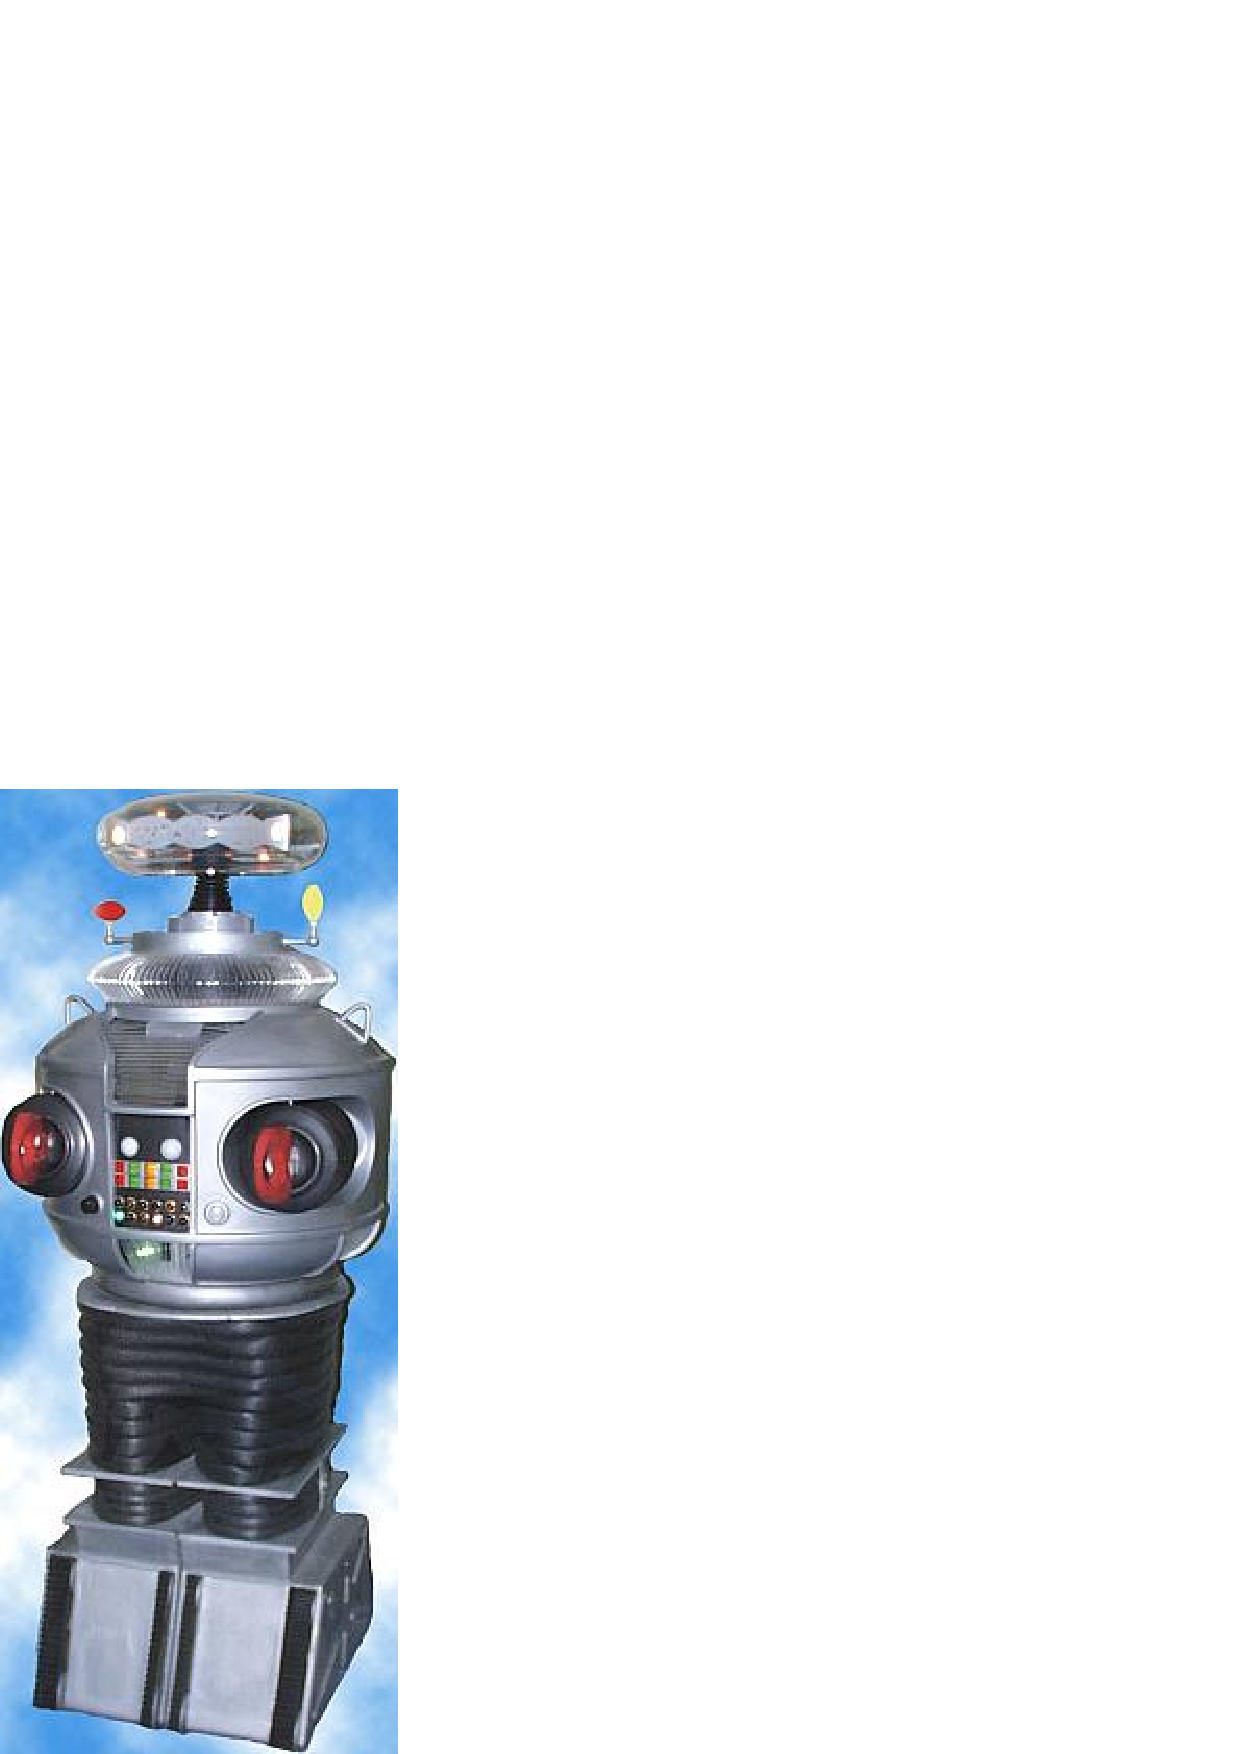
\includegraphics[scale=.35]{robot_lis}}%
\makebox[0pt][l]{\unhcopy0}%
\pushButton[\autoCenter{n}\BC{}\BG{}\S{S}\H{N}\textColor{0 0 1 rg}\TU{I'm robot man! Beep. Beep.}
    \AA{\AAMouseEnter{\JS{%
        if ( tts.available ) {\r\t
            tts.speaker = tts.getNthSpeakerName(0);\r\t
            tts.qText(event.target.userName);\r\t
            tts.talk();\r
        }
    }}}
]{robotman}{\the\wd0}{\the\ht0}}\\[1ex]
\textsf{\textbf{\textcolor{blue}{Robot man}}}

\pushButton[\CA{Robot man speaks}\A{\JS{robotTalks()}}]{robotmanspeaks}{}{12bp}

\end{center}

\smash{\makebox[0pt][l]{\href{http://www.acrotex.net}{
\includegraphics[scale=.2,angle=90]{AeB_Logo}}}}



\end{document}
